%!TEX root = ../talk.tex

\section{MXNet}\label{sec:MxNet}

%%%

\frameinlbffalse

{
\usebackgroundtemplate{
\tikz[overlay,remember picture] \node[opacity=0.8, xshift=-3.5cm, at=(current page.east)] {

\includegraphics[width=0.35\paperwidth]{figures/mxnet_logo.jpg}
};}

\begin{frame}[plain]
\frametitle{\S\ref{sec:MxNet}. \insertsection}
\listofframes
\end{frame}
\addtocounter{framenumber}{-1} % this page does not count

}

\frameinlbftrue

%%%
\subsection{Programming interface}
%%%

\begin{frame}
  \MyLogo
  \frametitle{General Comments}  

\begin{enumerate}
%
\item Support many different applications (e.g. computer vision, natural language processing,  speech recognition, unsupervised machine learning, support embedded APIs, visualization)
%
\item Mixed programming style: imperative and declarative
\begin{itemize}
\item Light-weighted (around 50K lines of core code)
\item Data parallelism with multi-devices: better scalability
\item Support many front-ends, including JavaScript (run on web browsers)
\item Provide intermediate-level and high-level interface modules
\item Provide abundant IO functions 
%
\end{itemize}
%
\item Fully compatible with Torch: modules and operators
%
\item Visualize neural network graphs
\begin{itemize}
\item Call mx.viz.plot\_network( )
\end{itemize}
%
\item Not well documented, code not easy to read
%
\end{enumerate}

\end{frame}

%%%
\subsection{Simple examples}
%%%

\begin{frame}[fragile]
  \MyLogo
  \frametitle{Example: SVM in MXNet}  

\begin{lstlisting}[language=python]
from __future__ import print_function  # make print compatible with python 2.x
import mxnet as mx
import numpy as np
from sklearn.datasets import fetch_mldata
from sklearn.decomposition import PCA
import matplotlib.pyplot as plt

import logging
logger = logging.getLogger()
logger.setLevel(logging.DEBUG)

# Symbolic network declaration. The following pattern was based on the article, 
# but feel free to play with the number of nodes and with the activation function
data = mx.symbol.Variable('data')
fc1  = mx.symbol.FullyConnected(data = data, name='fc1', num_hidden=512)
act1 = mx.symbol.Activation(data = fc1, name='relu1', act_type="relu")
fc2  = mx.symbol.FullyConnected(data = act1, name = 'fc2', num_hidden = 512)
act2 = mx.symbol.Activation(data = fc2, name='relu2', act_type="relu")
fc3  = mx.symbol.FullyConnected(data = act2, name='fc3', num_hidden=10)

# Here we add the ultimate layer based on L2-SVM objective
mlp = mx.symbol.SVMOutput(data=fc3, name='svm')
# To use L1-SVM objective, comment the line above and uncomment the line below
# mlp = mx.symbol.SVMOutput(data=fc3, name='svm', use_linear=True)

# Now we fetch MNIST dataset, add some noise, as the article suggests,
# permutate and assign the examples to be used on our network
mnist = fetch_mldata('MNIST original')
mnist_pca = PCA(n_components=70).fit_transform(mnist.data)
\end{lstlisting}

\end{frame}

\begin{frame}[fragile]
  \MyLogo
  \frametitle{Example: SVM in MXNet (Cont)}  

\ContinueLineNumber
\scriptsize{
\begin{lstlisting}[language=python]
# Add noise to the original data
noise = np.random.normal(size=mnist_pca.shape)
mnist_pca += noise

# Set seed for deterministic ordering
np.random.seed(1234) 
p = np.random.permutation(mnist_pca.shape[0])
X = mnist_pca[p]
Y = mnist.target[p]
X_show = mnist.data[p]

# Normalize the input to a value inside [0,1], and separate train and test sets
X = X.astype(np.float32)/255
X_train = X[:60000]
X_test = X[60000:]
X_show = X_show[60000:]
Y_train = Y[:60000]
Y_test = Y[60000:]

batch_size = 200 # Article's suggestion on batch size
train_iter = mx.io.NDArrayIter(X_train, Y_train, batch_size=batch_size)
test_iter = mx.io.NDArrayIter(X_test, Y_test, batch_size=batch_size)

# A quick work around to prevent mxnet complaining the lack of a softmax_label
train_iter.label= mx.io._init_data(Y_train,allow_empty=True,default_name='svm_label')
test_iter.label= mx.io._init_data(Y_test,allow_empty=True,default_name='svm_label')

\end{lstlisting}
}
\vskip 100pt

\end{frame}

\begin{frame}[fragile]
  \MyLogo
  \frametitle{Example: SVM in MXNet (Cont)}  

\ContinueLineNumber
\scriptsize{
\begin{lstlisting}[language=python]
# Here we instatiate and fit the model for our data
# The article suggests 400 epochs; we reduced to 10, for convenience
model = mx.model.FeedForward(
    ctx = mx.cpu(0),      # Run on CPU 0
    symbol = mlp,         # Use the network we just defined
    num_epoch = 10,       # Train for 10 epochs
    learning_rate = 0.1,  # Learning rate
    momentum = 0.9,       # Momentum for SGD with momentum
    wd = 0.00001,         # Weight decay for regularization
    )
    
model.fit(
    # Training data set
    X=train_iter,  
    # Testing data set. MXNet computes scores on test set every epoch
    eval_data=test_iter,  
    # Logging module to print out progress
    batch_end_callback = mx.callback.Speedometer(batch_size, 200)
    )  

plt.imshow((X_show[0].reshape((28,28))*255).astype(np.uint8), cmap='Greys_r')
plt.show()
print 'Result:', model.predict(X_test[0:1])[0].argmax()

# Now it prints how good did the network did for this configuration
print('Accuracy:', model.score(test_iter)*100, '%')\end{lstlisting}
}
%\vskip 100pt
\begin{center}
{\color{red}\scriptsize
https://github.com/dmlc/mxnet/blob/master/example/svm\_mnist/svm\_mnist.py
}
\end{center}

\end{frame}


%%%
\subsection{Visualization}
%%%

\begin{frame}
	\MyLogo
	\frametitle{Graph for example of SoftMax in MXNet}  
	
	\begin{figure}[htbp] 
		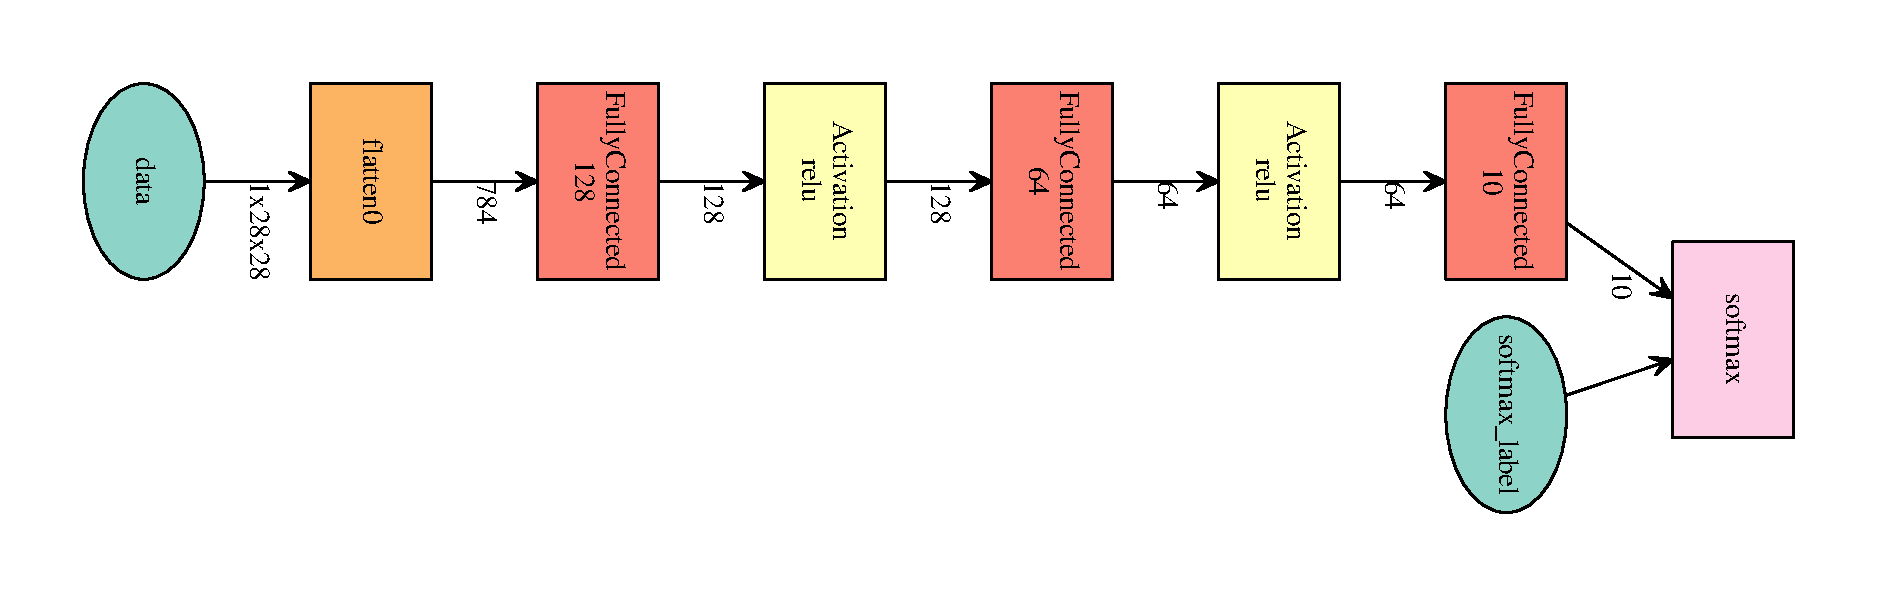
\includegraphics[width=\linewidth]{figures/mxnet_graph.pdf} 
	\end{figure}
	
\end{frame}